%In this section we provide details of the three datasets that we evaluate in this paper, as well as the methodology used.
\subsection{Dataset description}

\subsubsection{Email example (Malware detection)}
The first scenario evaluated in this article is related to the detection and analysis of malicious emails and therefore the detection of compromised user accounts. We assume having multiple emails, a spam classifier, and a display showing the graph of emails. We used ForceAtlas2, a Continuous Graph Layout Algorithm \cite{Jacomy2014} to get the locations of emails in the display (See Figure \ref{Fig:EnronData}).
We use the Enron email dataset, which has been made public by Cohen  \cite{Klimt2004}, and for which Shetty and Adibi \cite{Shetty2004} performed a set of
cleansing tasks, mainly by removing a large number of duplicate emails.  The final Enron dataset contains 252,759 emails sent from 17,527 users\footnote{http://www.ahschulz.de/enron-email-data/}.


\subsubsection{Twitter example (Detection of natural disasters)}
The second scenario is related to the detection and analysis of topical tweets on natural disasters. We assume having an agent monitoring tweets, a topical tweets classifier (e.g., \cite{Iman2017}), and a display showing the locations of the tweets (See Figure \ref{Fig:TwitterData}).  We used the  2.5 TB of Twitter data described in  \cite{Iman2017}, for which we restricted our analysis to the 9M tweets of January 2014.


\subsubsection{Reddit example (Detection of illegal transactions)}
The third scenario is related to the detection and monitoring of discussions related to deals of illegal merchandise on SilkRoad via Reddit. Here, we assume again having a monitoring agent, a classifier to classify discussions as being related to illegal transactions or not, and a display showing all discussions (we also use the ForceAtlas2 algorithm as shown in Figure \ref{Fig:RedditData}).
The Reddit dataset we used was crawled between October 2013 and January 2014, and contains 98,777 discussions.
%We provide more detailed statistics about the datasets described in
%Table~\ref{table:featureStatistics}. 



\begin{figure}[t]
\begin{centering}
\subfigure[Enron Networks.]{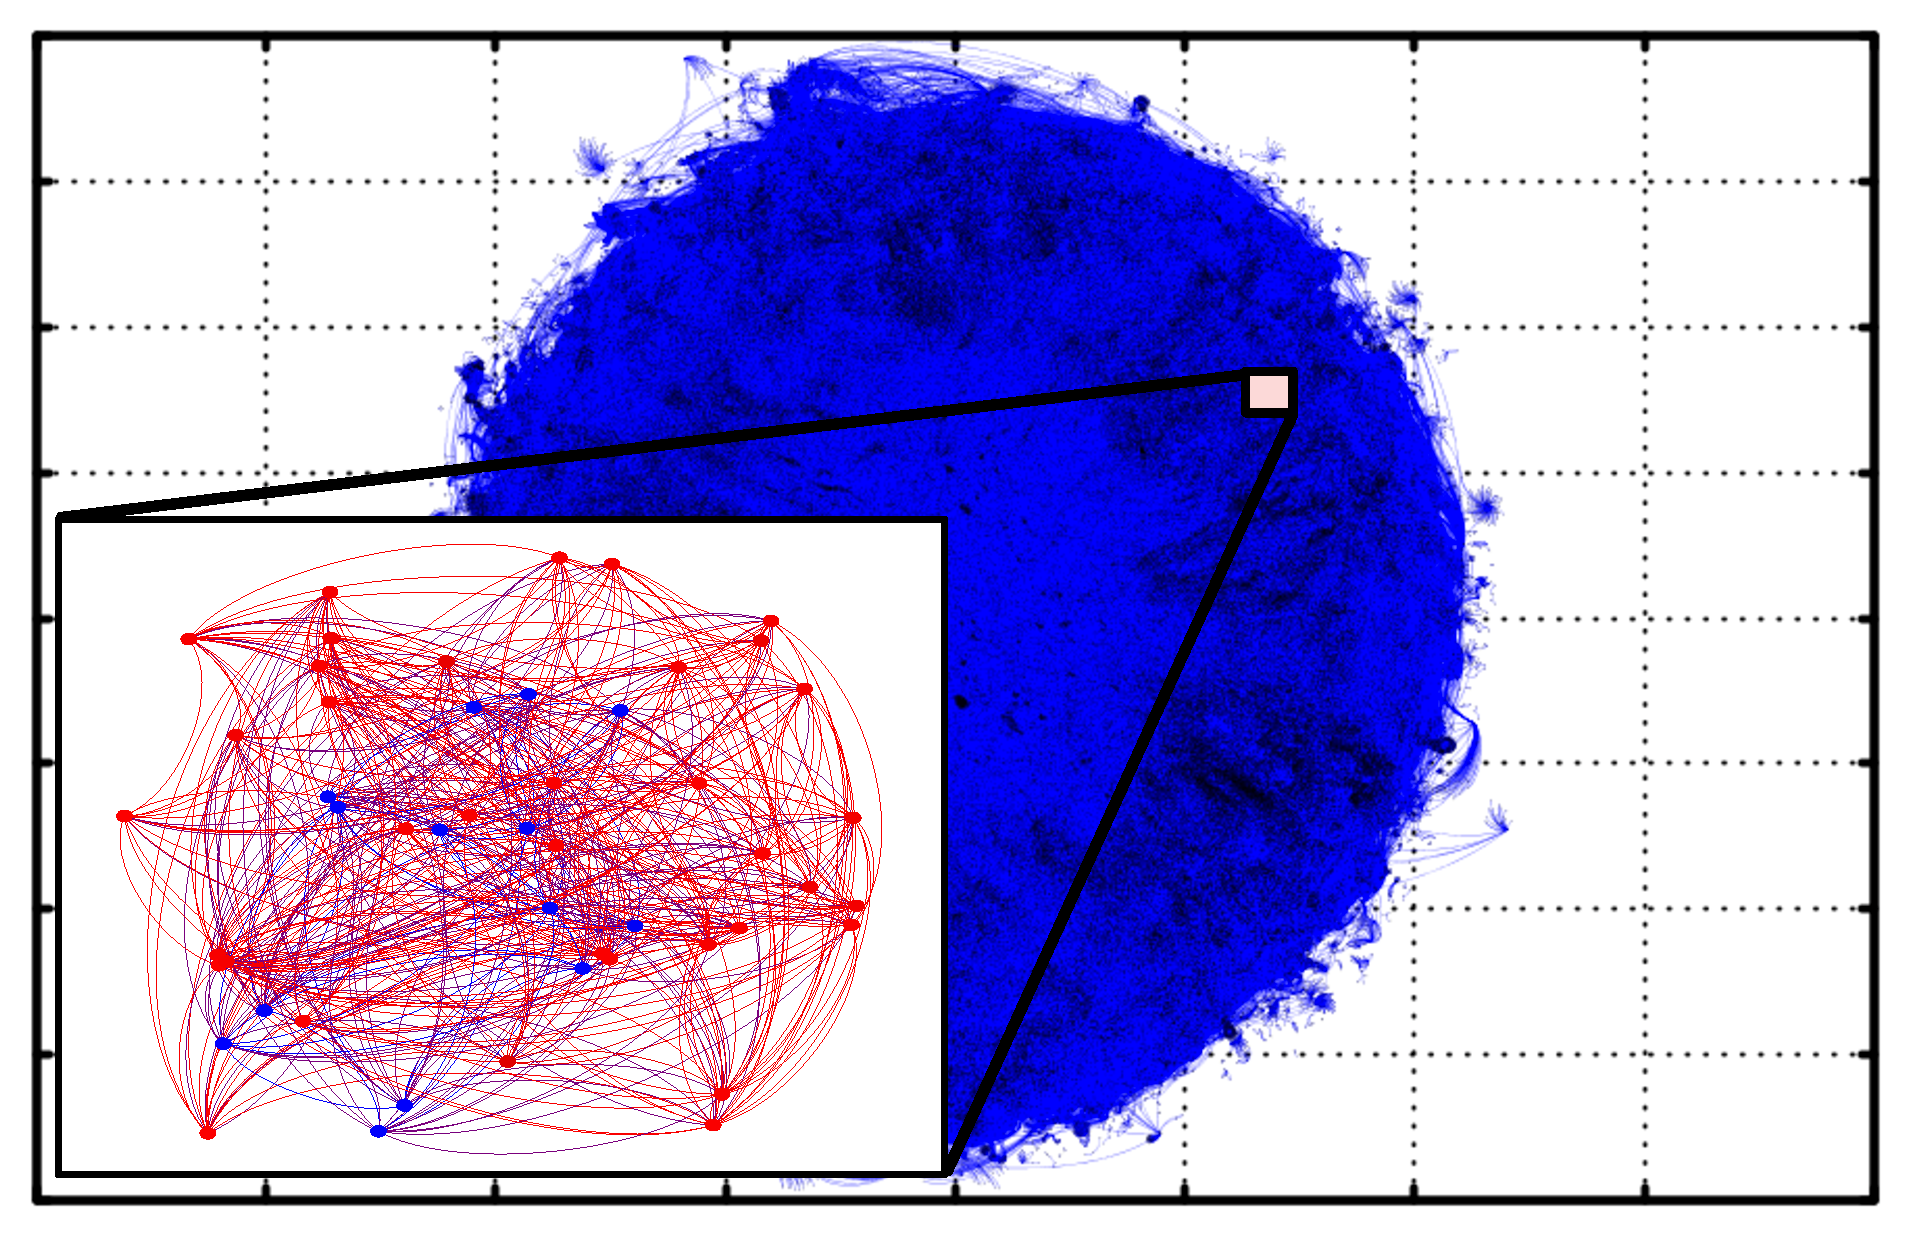
\includegraphics[width=2.8cm]{imgs/enron_net_4}\label{Fig:EnronData}}\subfigure[Twitter Networks.]{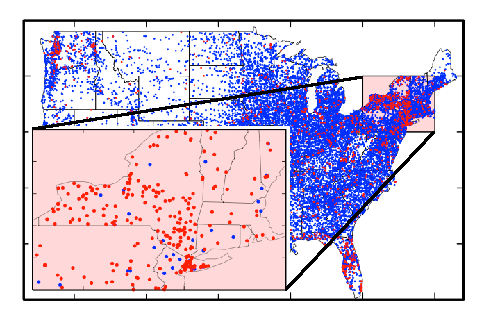
\includegraphics[width=2.8cm]{imgs/twitter_example_3}\label{Fig:TwitterData}}\subfigure[Reddit Networks.]{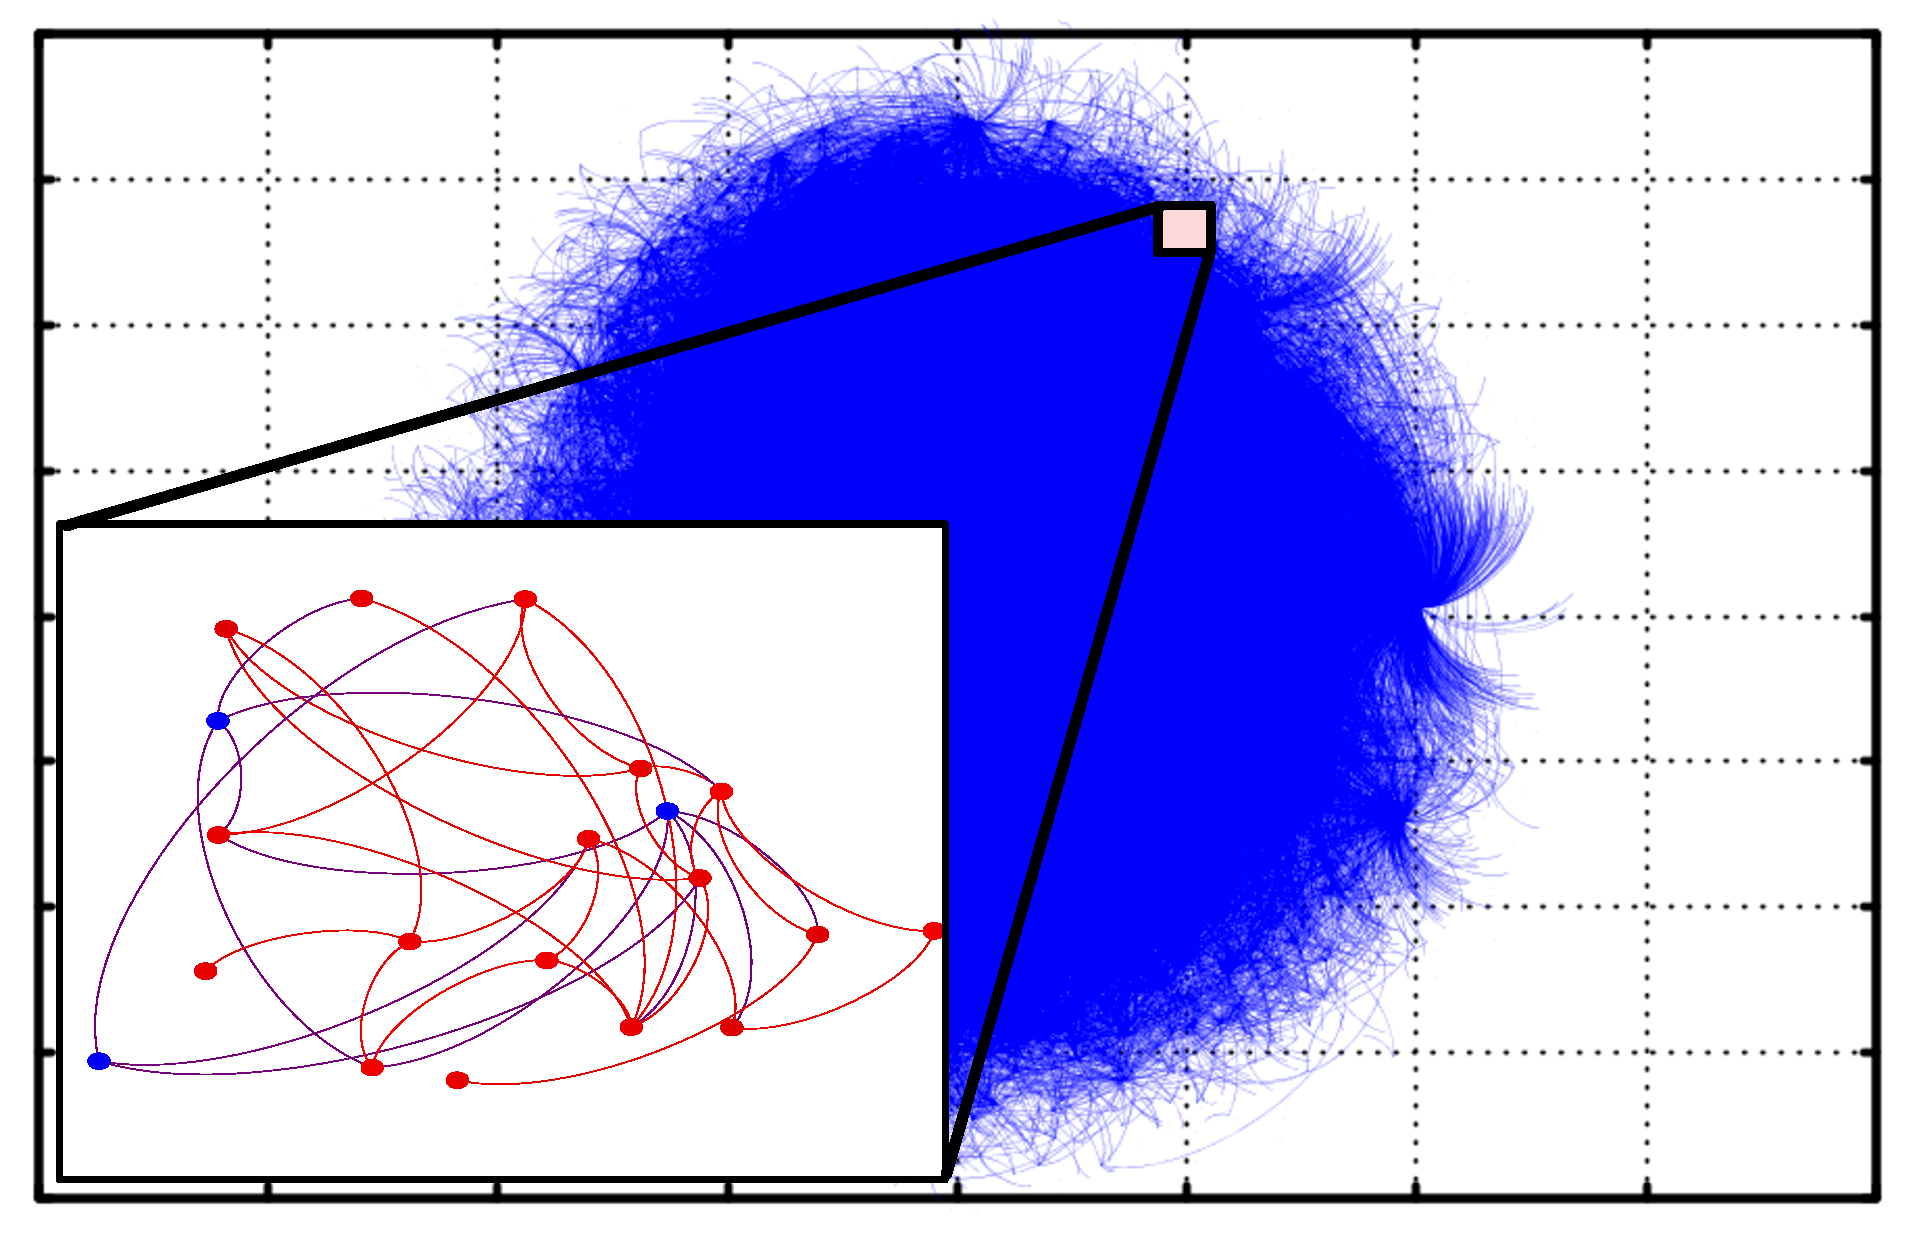
\includegraphics[width=2.8cm]{imgs/srforum3}\label{Fig:RedditData}}
\par\end{centering}
\caption{Layouts used for the different datasets.}
\end{figure}

\subsection{Evaluation methodology}

We assume that for each of the considered scenario,  we have a third party application-specific tool that predicts the probability score $S(i)$ that each information element is relevant in the context of that scenario, i.e., an email being malicious, a tweet being related to a natural disaster, or a discussion being related to an illegal transaction. This probability scoring function is task-specific and assumed to be given. 

For relevance prediction in our experiments, we use a noisy corruption of ground truth in order to synthetically evaluate a range of scenarios in terms of predicted relevance noise level.
We also explicitly vary the number of relevant information elements in our ground truth to assess performance variation as a function of class imbalance.  Hence, to setup a scenario with 20\% of relevant elements, we randomly select 20\% of the dataset and we assign a label value $l=1$ for each element in that set, and $l=0$ for each element out of that set. Then, for each element $j$, we assign the probability $S(j)$ of that element being relevant for scenario by introducing a random noise signal ratio as follows:
\begin{equation}
S(i) = \lambda*l+(1-\lambda)*r \; ,
\end{equation}
%we propose to simply randomly select an element $j$, 
%To simulate the 
%Finally, we propose to compute a global element score value $S(i)$ by introducing a noise signal ratio as follows:
where $r$ is a random noise value chosen with uniform distribution in the range $[0,1]$, and $\lambda$ is a weighting parameter  that satisfies $0.5 \leq \lambda \leq 1$, which controls the signal-to-noise ratio in the final probability value. Note that for $\lambda=1$, $S(j)$ gives the ground truth probability value (perfect classifier), whereas for $\lambda=0.5$, $S(j)$ returns a complete random probability value (random classifier).


For each dataset and given proportion of positive examples, the evaluation was carried out by averaging over 10 independent runs that each select random relevant documents according to the designated proportion.  We report the average ground truth F1-Score (i.e., ground truth is known in the experimental setting).



